%! suppress = TooLargeSection
%! suppress = SentenceEndWithCapital
%! suppress = TooLargeSection
% Preamble
\documentclass[11pt]{PyRollDocs}
\usepackage{textcomp}
\usepackage{csquotes}
\usepackage{wasysym}

\addbibresource{refs.bib}
% Document
\begin{document}

    \title{Gripping analysis PyRoll Plugin}
    \author{Christoph Renzing}
    \date{\today}

    \maketitle

    This plugin provides a gripping analysis based on the geometrical conditions inside the roll gap.


    \section{Model approach}\label{sec:model-approach}

    In contrary to flat rolling, the gripping analysis for grooves has to be done locally.
    This is the case, since the roll radius varies and therefore the gripping condition has to be checked locally.
    To archive a local spatial resolution of the roll gap in the x-z plane, the groove and profile are discretized into so called \enquote{Pillar Elements}.
    Since gripping is only possible in areas where the profile is larger than the grooves contour, this discretization is carried out inside the overlapping area.
    This area is defined by the intersection points between groove and incoming profile (see figure~\ref{fig:overlapping-intersection-points}).

    \begin{figure}
        \centering
        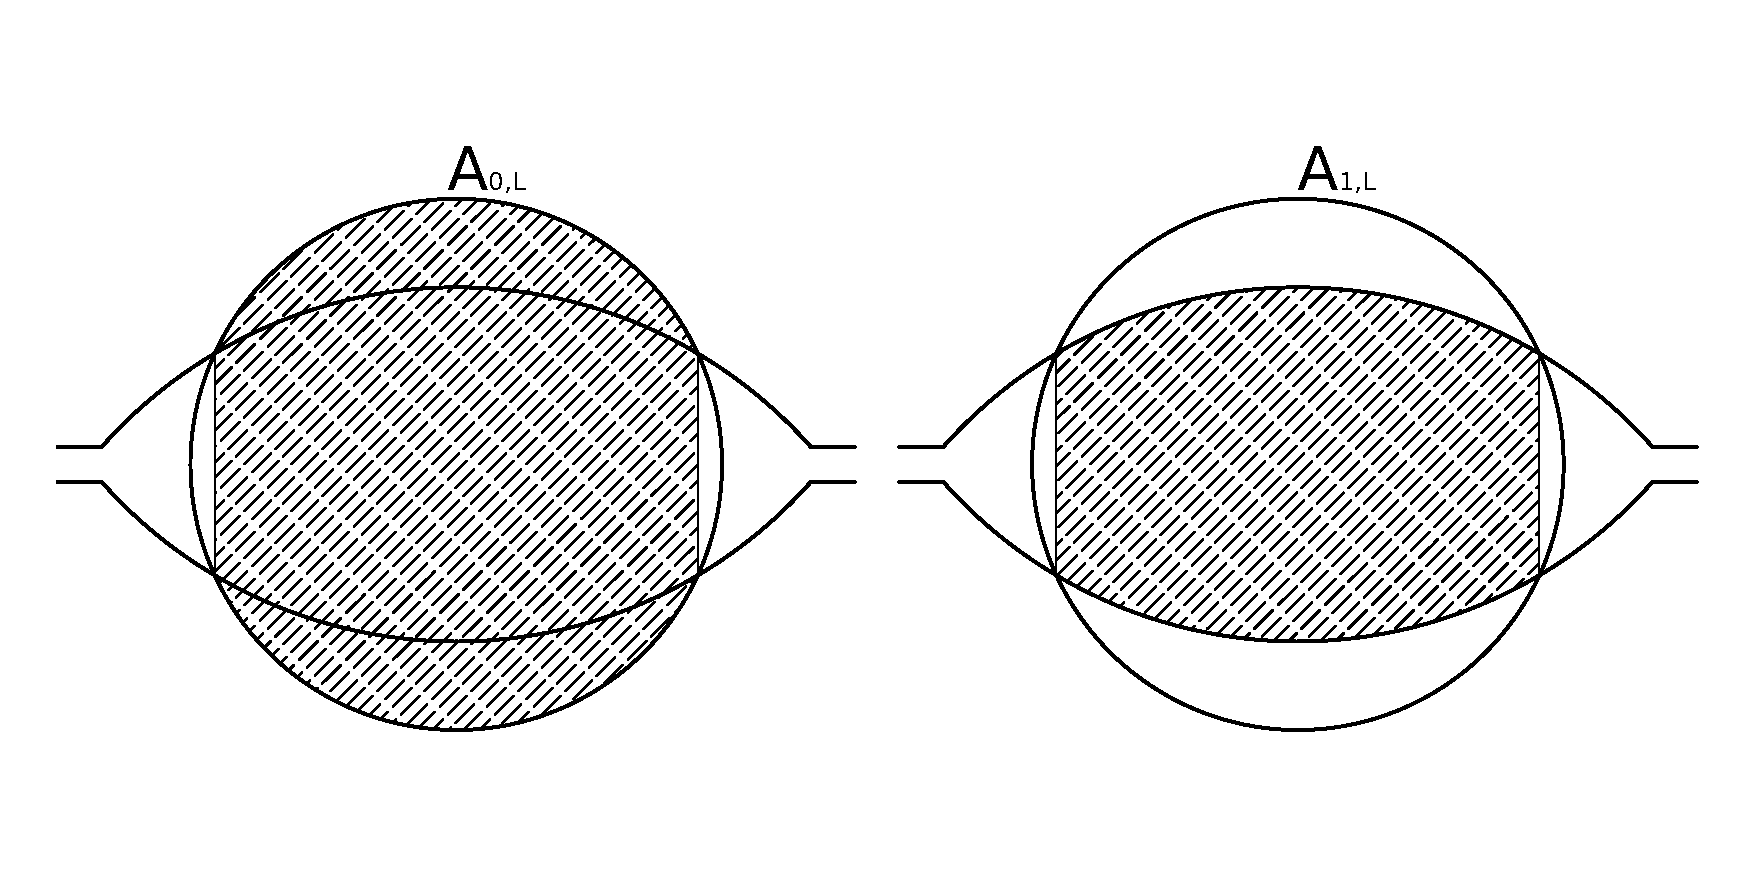
\includegraphics[width=.7\linewidth]{img/overlapping-area}
        \caption{Intersection points A to D for a round - oval roll pass}
        \label{fig:overlapping-intersection-points}
    \end{figure}

    Using the pilar elements, the local height change is calculated.
    For this, the \listinline{LineString} parts of the upper and lower groove and profile contour which are inside the pillars element boundary are interpolated and
    again discretized into 25 equidistant Points.
    From these points the local reduction is evaluated for the upper and lower part of the pillar (see figure ).
    Using the values, the arithmetic mean value of the reduction for the pilar element is calculated.
    After conducting this evaluation for all pillars, the point for the maximum height reduction in z - direction is searched using numpy.
    The resulting z-coordinate ($z(\Delta h = \Delta h_{max})$) is used to calculate the local radius of the work roll.
    This is done by subtracting the local grooves depth at the position and the nominal roll radius ($R_{gripping}$).
    Through this information,


    \section{Usage instructions}\label{sec:usage-instructions}

    The plugin can be loaded under the name \texttt{pyroll\_work\_roll\_elastic\_deformation}.
    Besides the hooks \lstinline{youngs_modulus}, the implemented \lstinline{body} hook is the entry point for the calculation.
    The calculation is done, using the classes \listinline{DiskElement}, \listinline{RollBody} and \listinline{MatrixMethod}.
    Several additional hooks on \lstinline{RollPass.Roll} are defined, which are used for calculation, as listed in \autoref{tab:hookspecs}.

    \begin{table}
        \centering
        \caption{Hooks specified by this plugin.}
        \label{tab:hookspecs}
        \begin{tabular}{ll}
            \toprule
            Hook name                        & Meaning                                                       \\
            \midrule
            \texttt{matrix\_method\_results} & Results of the matrix method as an array of arrays            \\
            \texttt{disk\_elements}          & Array of disk elements used for discretization of the grooves \\
            \texttt{deflection}              & Array of the deflection                                       \\
            \texttt{inclination}             & Array of the inclination                                      \\
            \texttt{bending\_moment}         & Array of the bending moment                                   \\
            \texttt{shear\_force}            & Array of the shear force                                      \\


            \bottomrule
        \end{tabular}
    \end{table}

    \printbibliography


\end{document}